\documentclass[11.5pt]{sig-alternate} % sets document style to sig-alternate
% packages
% typesetting
%\usepackage{dirtytalk} % typset quotations easier (\say{stuff})
\usepackage{hanging} % hanging paragraphs
\usepackage[defaultlines=3,all]{nowidow} % avoid widows
\usepackage[pdfpagelabels=false]{hyperref} % produce hypertext links, includes backref and nameref
\usepackage{xurl} % defines url linebreaks, loads url package
\usepackage{microtype}
%\usepackage[super]{nth} % easily create superscript ordinal numbers with \nth{x}
\usepackage{textcomp}
\newcommand{\texttildemid}{\raisebox{0.4ex}{\texttildelow}}
% layout
%\usepackage{enumitem} % control layout of itemize, enumerate, description
\usepackage{fancyhdr} % control page headers and footers
\usepackage{float} % improved interface for floating objects
%\usepackage{multicol} % intermix single and multiple column pages
% language
\usepackage[utf8]{inputenc} % accept different input encodings
\usepackage[english]{babel} % multilanguage support
% misc
\usepackage{graphicx} % builds upon graphics package, \includegraphics
%\usepackage{lastpage} % reference number of pages
%\usepackage{comment} % exclude portions of text (?)
\usepackage{xcolor} % color extensions
\usepackage[backend=biber, style=apa]{biblatex} % sophisticated bibliographies % necessary for HTML to display author info and date on abstract page
\usepackage{csquotes} % advanced quotations, makes biblatex happy
\usepackage{authblk} % support for footnote style author/affiliation
% tables and figures
\usepackage{tabularray}
%\usepackage{array} % extend array and tabular environments
\usepackage{caption} % customize captions in figures and tables (rotating captions, sideways captions, etc)
%\usepackage{cuted} % allow mixing of \onecolumn and \twocolumn on same page
\usepackage{multirow} % create tabular cells spanning multiple rows
%\usepackage{subfigure} % deprecated, support for manipulation of small figures
%\usepackage{tabularx} % extension of tabular with column designator "x", creates paragraph-like column whose width automatically expands
%\usepackage{wrapfig} % allows figures or tables to have text wrapped around them
%\usepackage{booktabs} % better rules
% dummy text
%\usepackage{blindtext} % blind text dummy text
%\usepackage{kantlipsum} % Kant style dummy text
\usepackage{lipsum} %lorem ipsum dummy text
% other helpful packages may be booktabs, longtable, longtabu, microtype

\pagestyle{fancy} % sets pagestyle to fancy for fancy headers and footers

% header and footer
% modern way to set header image
\renewcommand{\headrulewidth}{0pt} % defines thickness of line under header
\renewcommand{\footrulewidth}{0pt} % defines thickness of line above header
\setlength\headheight{80.0pt} % sets height between top margin and header image, effectively moves page contents down
\addtolength{\textheight}{-80.0pt} % seems to affect the lower height. maybe only works properly if footer numbers enabled?
\fancyhf{}
\fancyhead[CE, CO]{
\includegraphics[width=\textwidth]{headerImage.png}}
% footer
%\fancyfoot[LE,LO]{Article Title Here \\ DOI: }% left footer article title and doi
%\fancyfoot[CE,CO]{{}} % center footer empty
%\fancyfoot[RE,RO]{\thepage} % right footer page numbers
%\pagenumbering{arabic} % arabic (1, 2, 3) numbering in footer

\hypersetup{colorlinks=true,urlcolor=blue} % sets link color to blue
\urlstyle{same} % sets url typeface to same as rest of text

% set caption and figure to italics, label bold, left align captions, does not transfer to HTML
\captionsetup{labelfont=bf, font={large, it}, justification=raggedright, singlelinecheck=false}
\renewcommand\theContinuedFloat{\alph{ContinuedFloat}}

%this next bit is confusing, but essentially changes the width of the abstract. Seems to have been copied from this https://tex.stackexchange.com/questions/151583/how-to-adjust-the-width-of-abstract
\let\oldabstract\abstract
\let\oldendabstract\endabstract
\makeatletter %changes @ catcode to enable modification (in parsep)
\renewenvironment{abstract} %alters the abstract environment
{\renewenvironment{quotation}%
               {\list{}{\addtolength{\leftmargin}{1em} % change this value to add or remove length to the the default ?
                        \listparindent 1.5em%
                        \itemindent    \listparindent%
                        \rightmargin   \leftmargin%
                        \parsep        \z@ \@plus\p@}%
                \item\relax}%
               {\endlist}%
\oldabstract}
{\oldendabstract}
\makeatother %changes @ catcode to disable modification

% checks
% italics
% links
% dashes
% tildes
% dollars
\begin{document}

\title{A Universal Design for Robotics Education}

\author[1]{\large \color{blue}Mustafa Şahin Bülbül}

\affil[1]{Kafkas University, Kars, Turkey}

\toappear{}
%% ABSTRACT
\maketitle
\begin{@twocolumnfalse} 
\begin{abstract}
\item 
\textit{In this century, technological and educational needs increase drastically. Out of local language, educators need to teach robotic language and use necessary technologies to design robots like with the Arduino set.  Users may develop their own robots with this set. It also improves design and implementation skills. However, it is not a suitable design for blind learners. The universal design approach suggests educators to design courses in a way that meets the needs of all participants. By this approach, learning environments are helpful and useful for participants with special needs. With the scope of the study, we suggest a three step course design for robotics education; introducing with appropriate materials, using real materials with descriptions and discussing for further designs. In the first step, larger materials with big holes and components will be used to make sense of the devices. In the second step, while the sighted learners are testing we suggest educators describe what is happening in the activity. The last step is about imagination for what we should do more. The present study may lead to new insights on how to introduce systems to facilitate the learning process for blind students.}
\\ \\
Keywords: 
\end{abstract}
\end{@twocolumnfalse}

%% AUTHOR INFORMATION

\textbf{*Corresponding Author, Mustafa Şahin Bülbül}\\
\href{mailto:  msahinbulbul@gmail.com }{(msahinbulbul@gmail.com )} \\
\textit{Submitted  Nov 8 2016 }\\
\textit{Accepted  Jan 3 2017} \\
\textit{Published online  Feb 16 2017} \\
\textit{DOI:10.14448/jsesd.08.0005} \\
\pagebreak
\clearpage
\begin{large}
\section*{INTRODUCTION}

Education is a form of communication where all parts interact with each other.  However, communication problems such as having different languages can affect this interaction.  Therefore, humans develop a common language or “code” for computers to solve this problem.  Computers “communicate” with each other using these codes.  Out of computing input data based on written formulas, today, computers can collect data with sensors or coordinate some moving objects called “robots”.  Each user may design a robot if he/or she knows the codes, circuits and how to combine of them. 

Robots are human assistants that behave though codes.  However, combining codes and related hardware and circuits is a complex process. Some educators have focused on how to teach building robots online (Kuzucuoglu \& Erdemir, 2011), using cloud computers (Sell, Seiler \& Ptasik, 2012) or by using LEGOs which make connecting computer and other hardware easy (Zhao, Tan, Wen \& Guo, 2008).  In this study, Arduino set is used for robotics education.  It is a more popular, adaptive and open-source technology that, from beginners to experts, any student may learn by the use of it and its guides (Buechley, Eisenberg, Catchen \& Crockett, 2009; Kato, 2010). 
 
In this study, components of this set are explained for blind learners in terms of universal design.  For this purpose, models are designed for all components of the Arduino set.  Each model was designed with the expectation that the blind/low-vision learners can learn robotics more easily.  The term “universal design” is used for designs appropriate for all users with diverse usages.  It is known with seven principles: Equitable Use; Flexibility in Use; Simple and Intuitive Use; Perceptible Information; Tolerance for Error; Low Physical Effort; and, Size and Space for Approach and Use.  Bülbül (2015) proposed a useful application of this set.  He summarized universal design principles and provided materials to show its accessible and flexible usage.  This study is an example of using universal method for robotics education.

\section*{UNIVERSAL METHOD FOR ROBOTICS EDUCATION}
 
Universal method for robotics education (UMRE) explains three important levels (figure 1).  First, the educator should give a large and basic model of real components.  These models should be prepared with everyday materials.  This level is titled “introduction with model”. Educators should introduce how to build a robot with the set.  In this level both sighted and blind learners may use and have an experience with models.
 
\begin{figure}[ht]
     \centering
     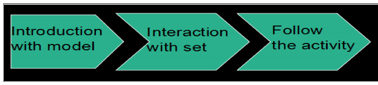
\includegraphics[width=1\linewidth]{fig1.png}
     \caption{Three level of Universal method for robotics education (UMRE)}
 \end{figure} 

In the second level, “interaction with set/models”, educators should give the real set piece by piece to both types of learners.  Let learners touch and listen to the introduction for the second time.  After these two levels, both sighted and blind learners should understand the components of the set and their relationships.  Sighted learners may learn more from the second level but the first level allows blind/low-vision learners to listen more than one and prepare for the second one.  After introducing the set, educators manage a building process of robots.  In this second level, sighted learners should combine and integrate the components but also describe what he or she is doing out loud.  Blind/low-vision learners should follow the building a robot activity with sighted friend’s explanations.  In this way, the first level makes the set flexible and the second level makes it accessible for blind/low-vision learners. 

In the third level, “follow the activity”, educators should give some braille documents of codes and some tactile figures of last positions of the set while sighted friends describe what he or she does and reads what he or she sees on the screen.  In this last level, the sighted learner and the educator should listen and answer the blind learner’s questions. 

Be aware that educators should be careful not to present original materials in the first level, due to the possibility that sighted learners might focus on the originals and resist listening to the explanations about models.  This indifference may subsequently affect blind learners’ attention and motivation. 

\subsection*{Preparing Models}

Models are prepared for the original parts of the robotic set using everyday materials such as rope, sticks and styropor (figures 2, 3 and 4). At first, the possibility of destroying the original parts of a set may be stressful to the learner.  However, models which are bigger and cheaper than the originals might motivate learner inquiry in an independent way. 

Blind learners cannot understand light emitting diodes (LEDs) due to their small and otherwise meaningless shape, but educators may make a bigger model of LED using pipette and small plastic jar (figure 3).  With the help of this basic model, educators expand the understanding of blind learners. 
 
\begin{figure}[ht]
     \centering
     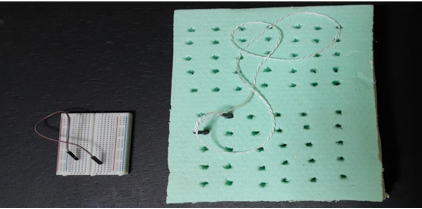
\includegraphics[width=1\linewidth]{fig2.png}
     \caption{Widely used circuit board (left) and its model for blind/low-vision learners (right)}
 \end{figure} 

\begin{figure}[ht]
    \centering
    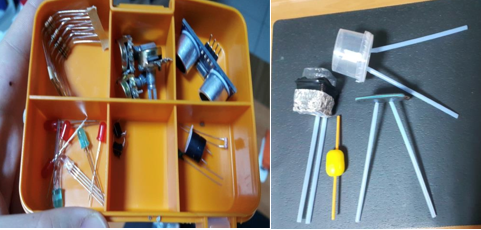
\includegraphics[width=1\linewidth]{fig3.png}
    \caption{Real circuit elements (left) and their models for blind/low-vision learners (right) }
\end{figure}
  
\begin{figure}[!ht]
    \centering
    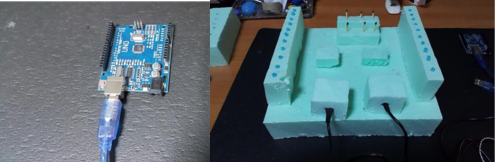
\includegraphics[width=1\linewidth]{fig4.png}
    \caption{Traditional circuit board (left) and model used for blind users (right) }
\end{figure}
\newpage

Educators may prepare models with similar colors to the original ones. This modification helps sighted learners’ understanding (Equitable usage).  Moreover, “Tolerance for Error” and “Low Physical Effort” are two principles of universal design.  So, by using these huge models educators support wrong usage at the beginning and allow the wiring of original set easily. 

\section*{CONCLUSION}

Receiving an education is a human right, so blind learners should benefit from education facilities as do their sighted peers.  In this perspective, blind learners also may learn robotics.  This is the responsibility of educators to prepare appropriate models and follow an appropriate methodology such as UMRE.  Nobody knows what a blind learner can do if he or she learns how to build a robot and no one limits these blind learners’ rights. This model can also be a good learning method for ensuring the opportunity and demonstrating that sighted and blind learners can work together.  Additionally, it is clear that UMRE is not only appropriate for robotics education.  Other laboratory activities and demonstrations may be done utilizing this method. 


\end{large}
\clearpage
\section*{REFERENCES}\par 

\leftskip 0.25in
\parindent -0.25in 
Buechley, L., Eisenberg, M., Catchen, J., \& Crockett, A. (2008, April). The LilyPad Arduino: using computational textiles to investigate engagement, aesthetics, and diversity in computer science education. In \textit{Proceedings of the SIGCHI conference on Human factors in computing systems} (pp. 423-432). ACM.

Bülbül, M. Ş., (2015). Öğreşme Sürecinde Evrensel Tasarım İlkeleri ile Fen Öğretiminde Engellilere Uyumlu Yöntem ve Materyal Örnekleri. \textit{Sürdürülebilir ve Engelsiz Bilim Eğitimi, 1}(0), 1-18.

Kato, Y. (2010, January). Splish: a visual programming environment for Arduino to accelerate physical computing experiences. In \textit{2010 Eighth International Conference on Creating, Connecting and Collaborating through Computing} (pp. 3-10). IEEE. 

Kuzucuoglu, A. E., \& Erdemir, G. (2011). Development of a web-based control and robotic applications laboratory for control engineering education. \textit{Information technology and control, 40}(4), 352-358.

Sell, R., Seiler, S., \& Ptasik, D. (2012). Embedded system and robotic education in a blended learning environment utilizing remote and virtual labs in the cloud, accompanied by Robotic HomeLab Kit ‘. \textit{International Journal of Emerging Technologies in Learning, 7}(4), 26-33. 

Zhao, S., Tan, W., Wen, S., \& Guo, C. (2008, December). Research on robotic education based on LEGO bricks. In \textit{Computer Science and Software Engineering, 2008 International Conference on} (Vol. 5, pp. 733-736). IEEE. 

\end{document}